\documentclass{report}


% Language + Document formatting
\usepackage[dutch]{babel}
\usepackage[a4paper,top=2cm,bottom=2cm,left=2cm,right=3cm,marginparwidth=1.75cm]{geometry}
\usepackage[indent=10pt]{parskip}

% Titles customization
\usepackage{titlesec}
\newcommand{\hsp}{\hspace{20pt}}
\titleformat{\chapter}[hang]{\Huge\bfseries}{\thechapter\hsp}{0pt}{\Huge\bfseries}


% Afbeeldingen
\usepackage{graphicx}
\usepackage{subcaption}
\graphicspath{ {./images/} }



\title{OnlyPaws}
\author{Mathijs Verbeure}

\begin{document}
\maketitle

\tableofcontents

\chapter{Inleiding}
De eerste vraag wanneer een project zo absurd als ``een dating platform voor katten'' gepresenteerd wordt is: \verb|Waarom?| Een concreet antwoord hierop\dots heb ik niet.
Toen het project voorgelegen werdt nam ik de beslissing om geen standard onderwerp te nemen. Kort door de bocht: niks saai.
Zo behoud ik mijn motivatie en valt de inspiratiestroom niet zo snel stil.
Een ander punt waar ik rekening mee nam was dat dit project, indien mooi afgerond, leuk op een CV / Portfolio kan komen. 
Kotlin is een snel evoluerende taal die veel gebruikt wordt binnen de Google-omgeving, en zeker toegepast kan worden binnen de context van een bedrijf.
Een topic kiezen die interessant is en waarover veel te bespreken valt is dus erg belangrijk; veel valt er niet te vertellen over een \verb|To-Do| app, maar een online dating app voor poezen? Dat lokt wel aandacht!

Dat zijn de officiële redenen voor dit project, maar er blijven er nog twee over die het meeste invloed gehad hebben op mijn beslissing. 
\begin{enumerate}
    \item Ik heb poezen graag; het zijn grappige beesten.
    \item Het is een grappig concept.
\end{enumerate}


\textit{OnlyPaws} is gebaseerd op \textit{Tinder}\texttrademark, het online dating platform. Hier kunnen gebruikers profielen bekijken van andere, naar rechts swipen indien de persoon hun interesseert en naar links indien niet.
Indien beide gebruikers naar rechts swipen --- zal ik verder ``Liken'' noemen --- dan is het een ``Match'', en kunnen ze berichten naar elkaar sturen om verder contact op te nemen.

Een vrij simpel concept dat enorm populair is geworden. Zelf had ik \textit{Tinder} nog nooit gebruikt, enkel via een vriend of het internet de groffe lijnen begrepen.
Om een app te ontwerpen hierrond moest ik uiteraard zelf eens uit proberen en notities nemen over de UI/UX.\@ De `testprocedure' was inzichtsvol en bracht verschillende ideeën op die ik zou proberen te integreren in mijn versie.
Sommige details in de UX vielen erg hard op, zoals bij voorbeeld hoe vaak er een voorstel komt om een subscriptie te nemen die je voordelen geeft. Eens je maandelijks betaal kan je berichten sturen zonder match --- via wat ze ``First Impressions'' noemen --- bekijken wie jouw profiel geliked heeft en meer.
Al zou het hilarisch zijn om tijdens de demonstratie niks te kunnen tonen omdat er betaald moet worden, dit zal ik voor overduidelijke redenen niet doen. 

De economische strategieën van techgiants zijn niet te bespreken in dit verslag. Dit is een project in academische context, geld-gerichte implementaties zijn dus niet gepast.
Verder nog, zelf vind ik dat bedrijven veel te gericht zijn op winst, niet op de producten die gemaakt worden; \textit{Tinder} valt amper te gebruiken door alle reclame die ingebouwd is.
Dit weiger ik op eender welke wijze te implementeren.

Deze negatieve kanten van het oorspronkelijk product zijn dus niet te vinden in dit project! Deze verschillen bespreek ik wel eens ze aan bod komen.


\chapter{Verloop}

Bij het openen van de app kom je terecht op de Login pagina en gaat Google's \textit{Credential Manager} open. Deze onthoudt welke gegevens al gebruikt zijn om in te loggen of te registreren.
Dankzij deze moet je je paswoord ook niet onthouden; het wordt allemaal veilig bewaard door Google.
De pop-up laat je selecteren welk account je wilt gebruiken als, stel maar, je meerdere katten hebt. Indien er geen credentials te vinden zijn wordt je automatisch naar de Register pagina verstuurd.
Verder kan je ook het Credentials menu sluiten om een gebruiker aan te maken.

Het proces om een gebruiker aan te maken neemt twee stappen, gesplitst over twee opeenvolgende paginas; eerst de belangrijke gegevens voor login, dan de informatie die andere gebruikers zullen zien.
Je vult een email in, gevolgd door een paswoord. Je mag door naar de volgende stap eens deze checks goedgekeurd zijn: het emailadress mag nog niet in de database bestaan en het paswoord moet meer dan 6 karakters lang zijn.
In een perfecte wereld zou een bevestigingsmail verstuurd worden, maar dat valt buiten de scope van dit project.

In de tweede pagina moet je een naam, beschrijving en afbeelding invullen, die andere gebruikers te zien krijgen. Er zijn geen beperkingen op deze, alleen ze mogen niet leeg zijn.
Hier komt de scope van dit project weer in spelen: ik maak gebruik van Firebase RealTime database om alle gegevens en authenticatie op te slaan. Hier kunnen geen afbeeldingen opgeslaan worden, alleen text/JSON.
Daarom zijn er op de RegisterDetails pagina twee knoppen; één om een afbeelding lokaal te openenen en één waarbij je de link naar een random foto online krijgt. 
Beide zijn volledig functioneel, maar de lokale afbeelding gaat door niemand buiten de huidige telefoon bekeken kunnen worden, dus raad ik niet aan.
De foto kan je aan de hand van een Android Intent selecteren.

Proficiat! U bent nu de trotse eigenaar van een OnlyPaws account en wordt doorgestuurd naar de Home pagina.
Hier worden één per één andere profielen getoond. Je kan ofwel Liken ofwel Disliken, door rechts of links te klikken op de pagina. 
Bij een nieuw account worden hulptekens gegeven die aanduiden welke kant correspondeert aan welke actie. Deze kan je uitschakelen door in het midden --- tussen de twee knoppen --- te klikken.
Centraal staat de foto van de kat met de naam en beschrijving bovenaan.
Elke profiel die geliked wordt komt in de Favorites pagina te staan. Hier kan je alle profielen van Liked naar Dislike sturen en omgekeerd, plus de foto's bekijken door op de thumbnail te klikken.
Bij het verwissellen van een profiel komt een pop-up tevoor om na te vragen of de gebruiker dit zeker wilt doen. Indien ja, wordt de operatie uitgevoerd. Indien nee sluit de pop-up en verandert er niks.

Ten laatste is er een Account pagina, waar de gebruikersgegevens aangepast kunnen worden. Een lokale foto opslaan kan nog niet, dus de profiel foto aanpassen is nog niet mogelijk, maar naam en beschrijving wel.
Voer de nieuwe text in, duuw op het knopje en de gegevens worden opgeslaan.
In de boven-rechtse hoek is een Log-Out knop te vinden waarmee je, uiteraard, kunt uitloggen van het account en terug naar de Login gaan.


\begin{figure}[h]
    \centering
    \begin{subfigure}[b]{0.32\textwidth}
        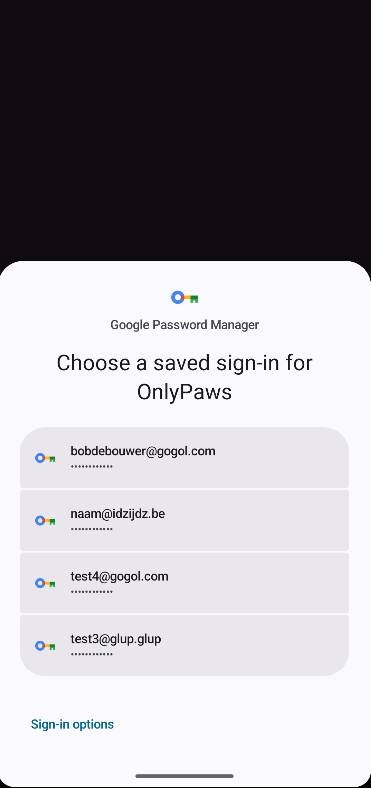
\includegraphics[width=\textwidth]{DEMO_login.png} 
        \caption{Credential Manager}
    \end{subfigure}
    \hfill
    \begin{subfigure}[b]{0.32\textwidth}
        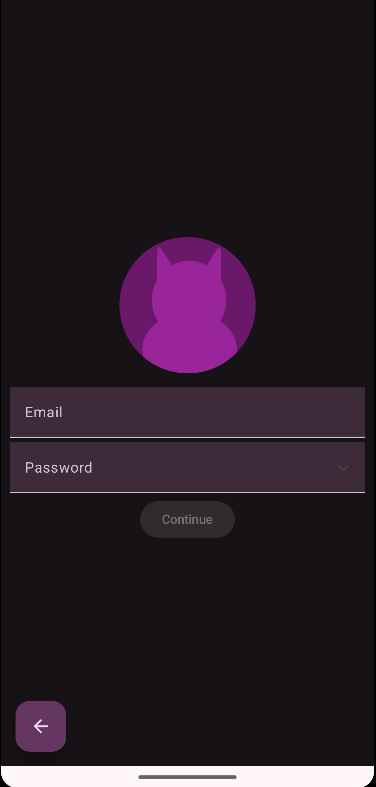
\includegraphics[width=\textwidth]{DEMO_Reg1.png} 
        \caption{Lege Register pagina}
    \end{subfigure}
    \hfill
    \begin{subfigure}[b]{0.32\textwidth}
        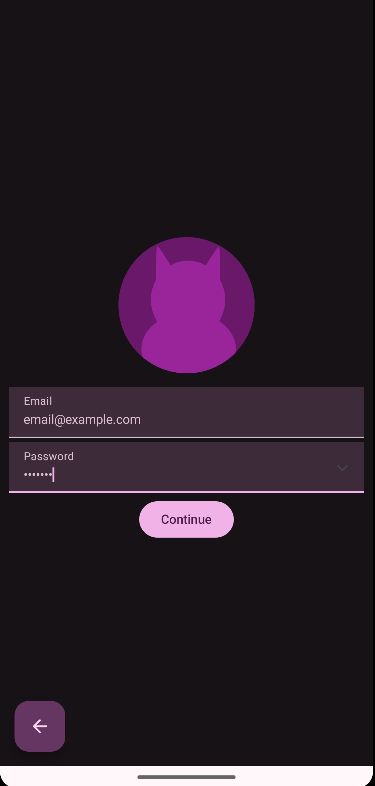
\includegraphics[width=\textwidth]{DEMO_Reg2.png} 
        \caption{\textit{Continue} eens ingevuld}
    \end{subfigure}

    \vspace{1em}

    \centering
    \begin{subfigure}[b]{0.32\textwidth}
        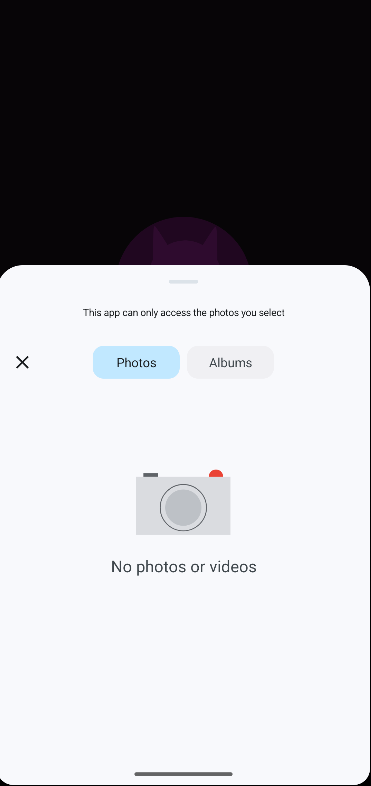
\includegraphics[width=\textwidth]{DEMO_RegSelect.png} 
        \caption{Afbeelding selecteren}
    \end{subfigure}
    \hfill
    \begin{subfigure}[b]{0.32\textwidth}
        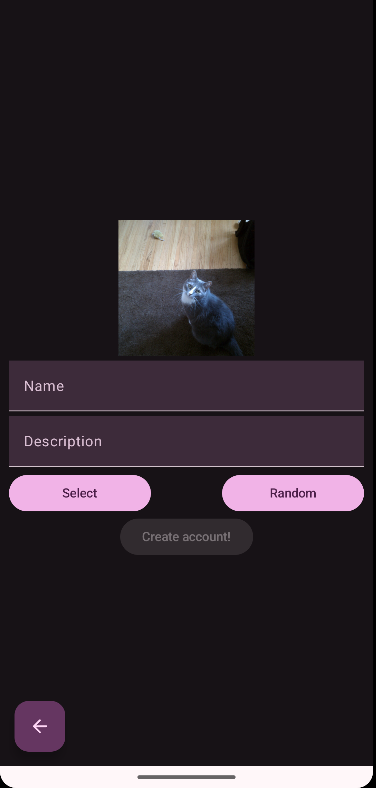
\includegraphics[width=\textwidth]{DEMO_RegRandom.png} 
        \caption{Random afbeelding}
    \end{subfigure}
    \hfill
    \begin{subfigure}[b]{0.32\textwidth}
        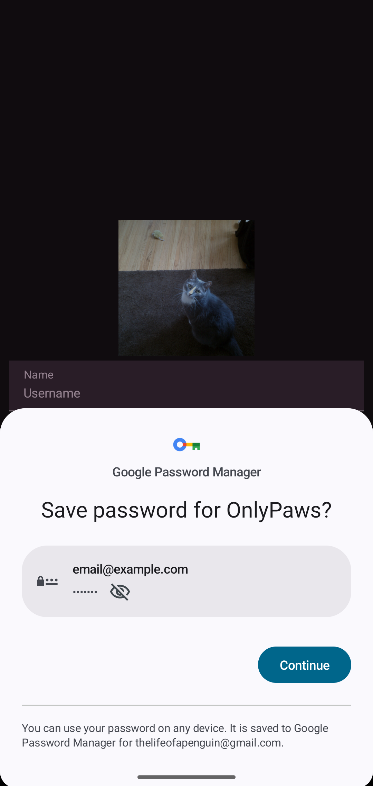
\includegraphics[width=\textwidth]{DEMO_RegSave.png} 
        \caption{Gegevens opslaan}
    \end{subfigure}

\end{figure}


\begin{figure}[h]

    \centering
    \begin{subfigure}[b]{0.32\textwidth}
        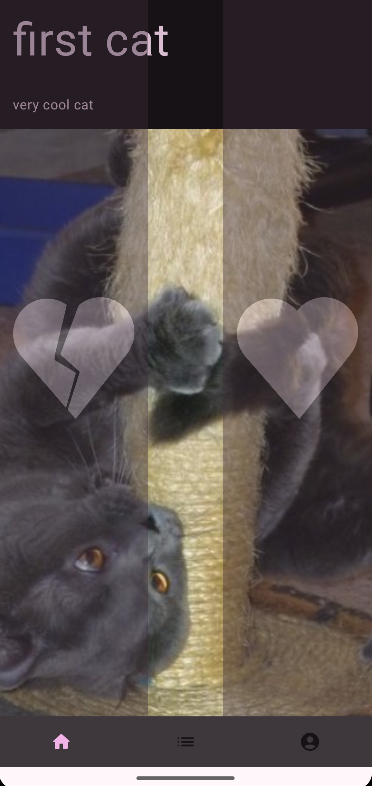
\includegraphics[width=\textwidth]{DEMO_Main1.png} 
        \caption{Main pagina}
    \end{subfigure}
    \hfill
    \begin{subfigure}[b]{0.32\textwidth}
        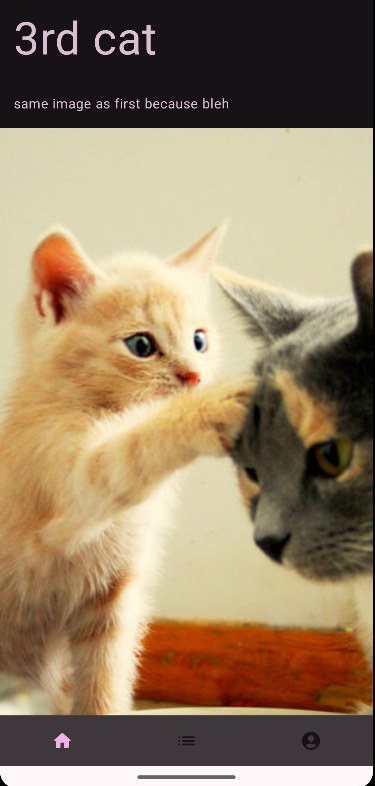
\includegraphics[width=\textwidth]{DEMO_Main2.png} 
        \caption{Nieuwe profiel na liken}
    \end{subfigure}
    \hfill
    \begin{subfigure}[b]{0.32\textwidth}
        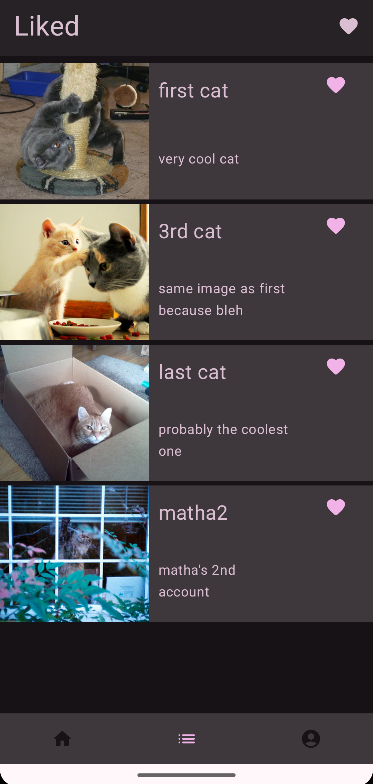
\includegraphics[width=\textwidth]{DEMO_List1.png} 
        \caption{Liked profielen}
    \end{subfigure}

    \centering
    \begin{subfigure}[b]{0.32\textwidth}
        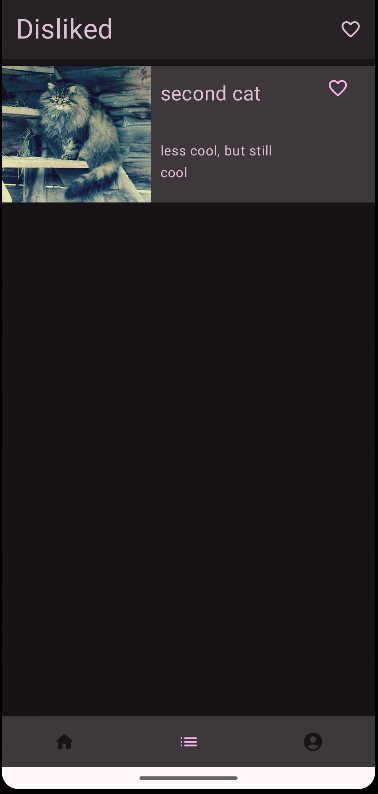
\includegraphics[width=\textwidth]{DEMO_List2.png} 
        \caption{Disliked profielen}
    \end{subfigure}
    \hfill
    \begin{subfigure}[b]{0.32\textwidth}
        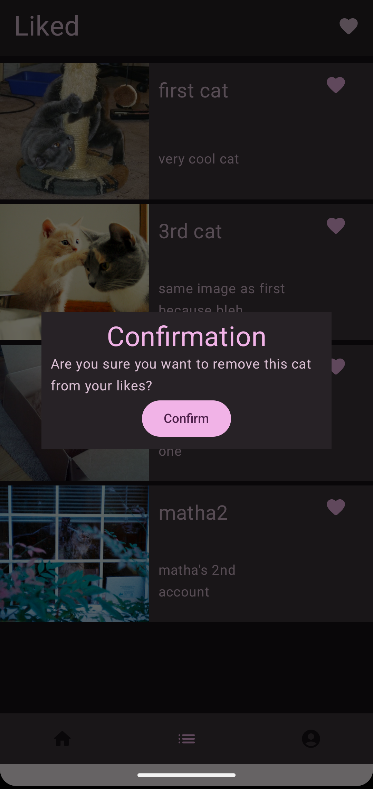
\includegraphics[width=\textwidth]{DEMO_List3.png} 
        \caption{Like veranderen}
    \end{subfigure}
    \hfill
    \begin{subfigure}[b]{0.32\textwidth}
        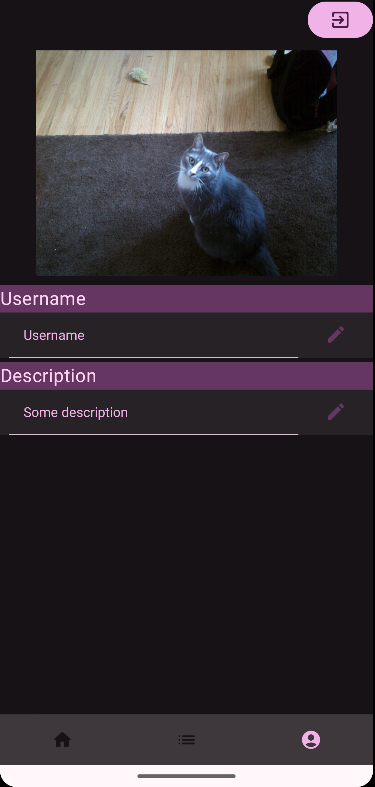
\includegraphics[width=\textwidth]{DEMO_Acc.png} 
        \caption{Account pagina}
    \end{subfigure}

\end{figure}

\begin{figure}[h]
    \centering
    \begin{subfigure}[b]{0.32\textwidth}
        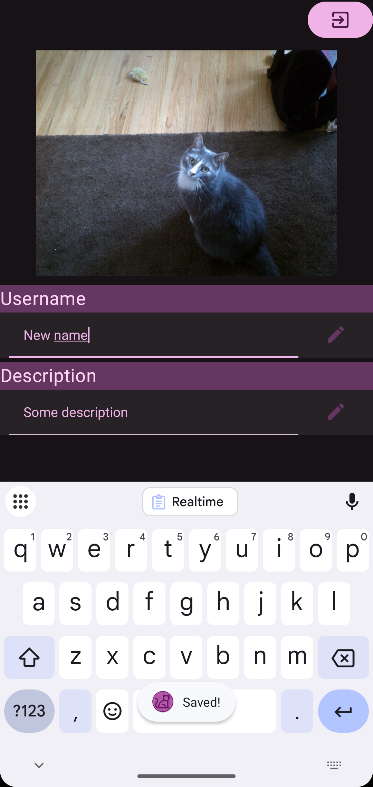
\includegraphics[width=\textwidth]{DEMO_Acc2.png}
        \caption{Gegevens aanpassen}
    \end{subfigure}
    \hfill
    \begin{subfigure}[b]{0.32\textwidth}
        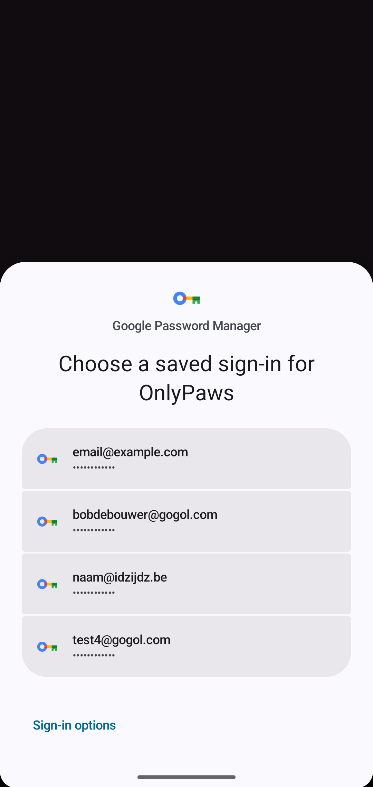
\includegraphics[width=\textwidth]{DEMO_Acc3.png}
        \caption{Terug naar Login}
    \end{subfigure}
    \hfill
\end{figure}





















\chapter{Documentatie}
\section{MVVM}
MVVM is een structuur waarbij er zo veel mogelijk abstractie is tussen data en display. 
Doorheen het creatieprocess is de structuur meerdere keren vanaf nul weer begonnen, vaak omdat ik een nieuwe manier van werken gevonden had en die voorkeur gaf over de oude methode.
Een van de belangrijkste concepten is het \textit{Separation of Concerns} principe. Dit legt voor dat elk object, elke classe, elke pagina, elk data model geen kennis mag hebben van waar het gebruikt wordt, of in welke toepassing het beland.
Eender welk bestand zou theoretisch geplakt kunnen worden in eender welke omgeving en werken. Een pagina zou geen fout moeten geven als een viewmodel verwisselt wordt.
De structuur die ik aangenomen heb voor dit project draait om een paar begrippen die bij elke toepassing opnieuw gemaakt worden, en op een robuste manier code veiligheid behalen.

\begin{center}
    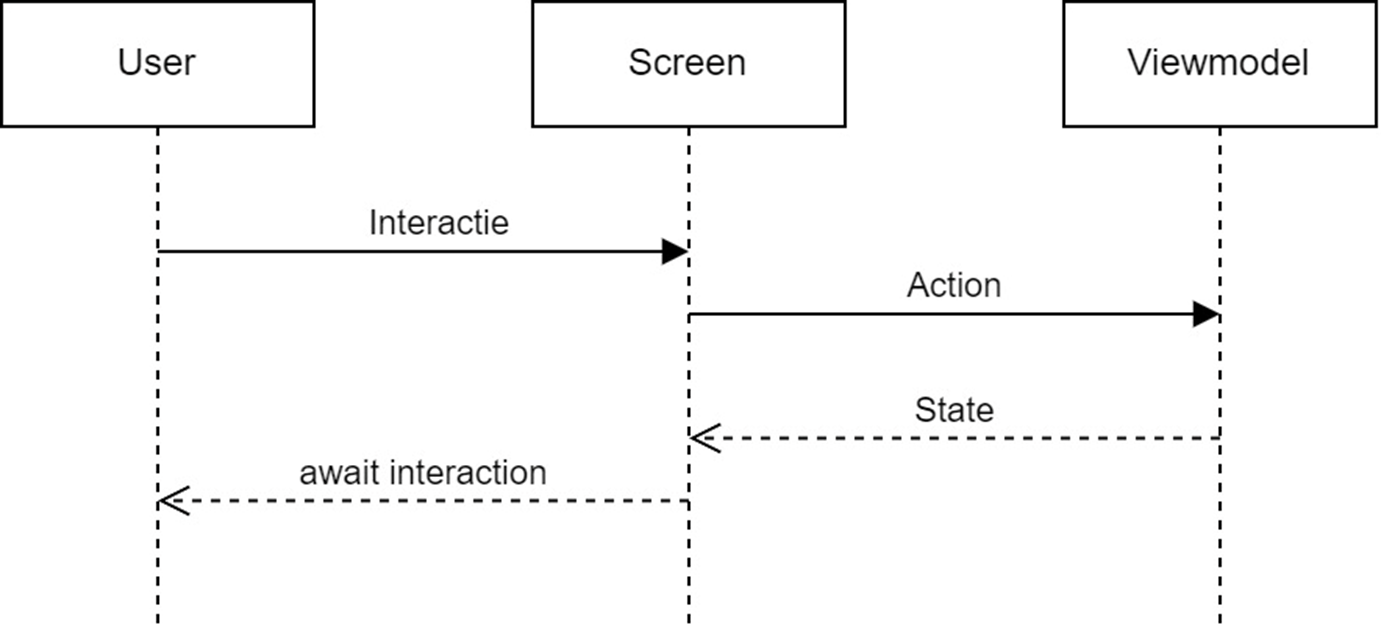
\includegraphics[scale=0.5]{MVVM_Overzicht}
\end{center}

\subsection{ViewModel}
Viewmodels zijn de classes waarin data wordt bijgehouden. Ze doen het rekenwerk, halen data op en sturen de nodige informatie door naar de gebruikersinterface.
Intern bestaan er meerdere variabelen die doorheen de levenstijd van het viewmodel geldig blijven, samen met de nodige functies om alles operationeel te krijgen.
Verder is er maar één publieke property (de \textit{ScreenState}) en één publieke methode (de \textit{OnAction} methode). Meer hierover in hun respectievelijke subsecties.

Het basis ViewModel classe heeft twee eigenschappen die nodig zijn voor hun verwachtte werking.
De eerste hiervan is dat ze niet composable zijn; hierdoor moet er geen \textit{remember} toegevoegd worden zodat ze heen de lifecycle van de applicatie blijven.
Dit werkt samen met de tweede eigenschap: ze volgen het singleton patroon. Dit garandeert dat elke nieuwe aanroeping van een VM identiek hetzelfde object zal geven.
Aan de hand van deze twee eigenschappen kunnen VMs doorheen de levenscyclus van de applicatie geldig blijven.

\begin{center}
    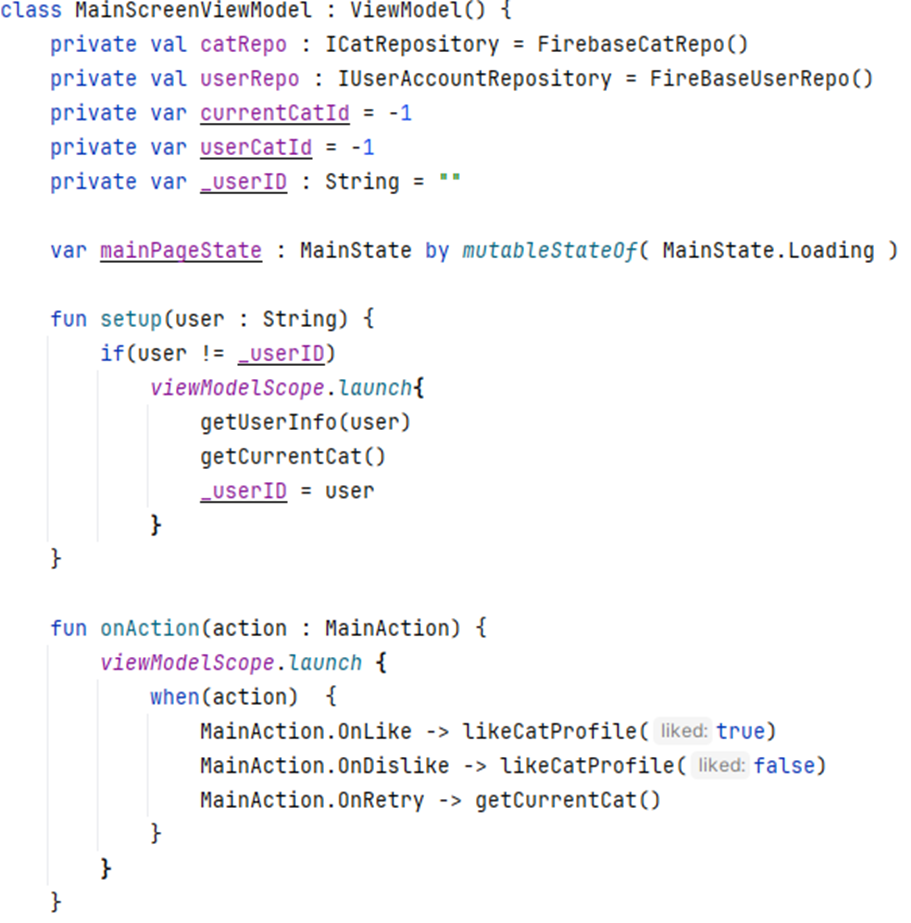
\includegraphics{MVVM_Viewmodel}
\end{center}


\subsection{Screen}
Screens vormen de omgeving waarmee de gebruiker kan interageren. Dit zijn de ``views'' van in het MVC patroon.
Het toont de gegevens op één manier ongeacht welke gegevens dit precies zijn. 
Al wat de Screen weet is dat er een dataset gegeven wordt in een zeker formaat en dat er een zeker stuk code uitgevoerd moet worden bij het klikken op de knop.
Nogmaals, dit is een manier om de taken binnen de applicatie te splitsen. Wat het klikken op een knop doet maakt de Screen volledig niets uit. Of dit een externe library ophaalt, data schrijft naar een bestand of een Toast aanmaakt is irrelevant.
Alles wat een component hoort te weten is dat er een functie bestaat bij het klikken van elke knop.

Aan de hand van de huidige state parameter wordt de correcte display vooruit gebracht.
Elke screen heeft één publieke constructor en verschillende privé constructoren die voor de verschillende scenario's dienen.
Zo zijn er standard een ``Success(value)'', ``Failure(error)'' en ``Loading()'', drie vaak voorkomende scenarios, voornamelijk wanneer er data opgehaald moet worden.

\begin{center}
    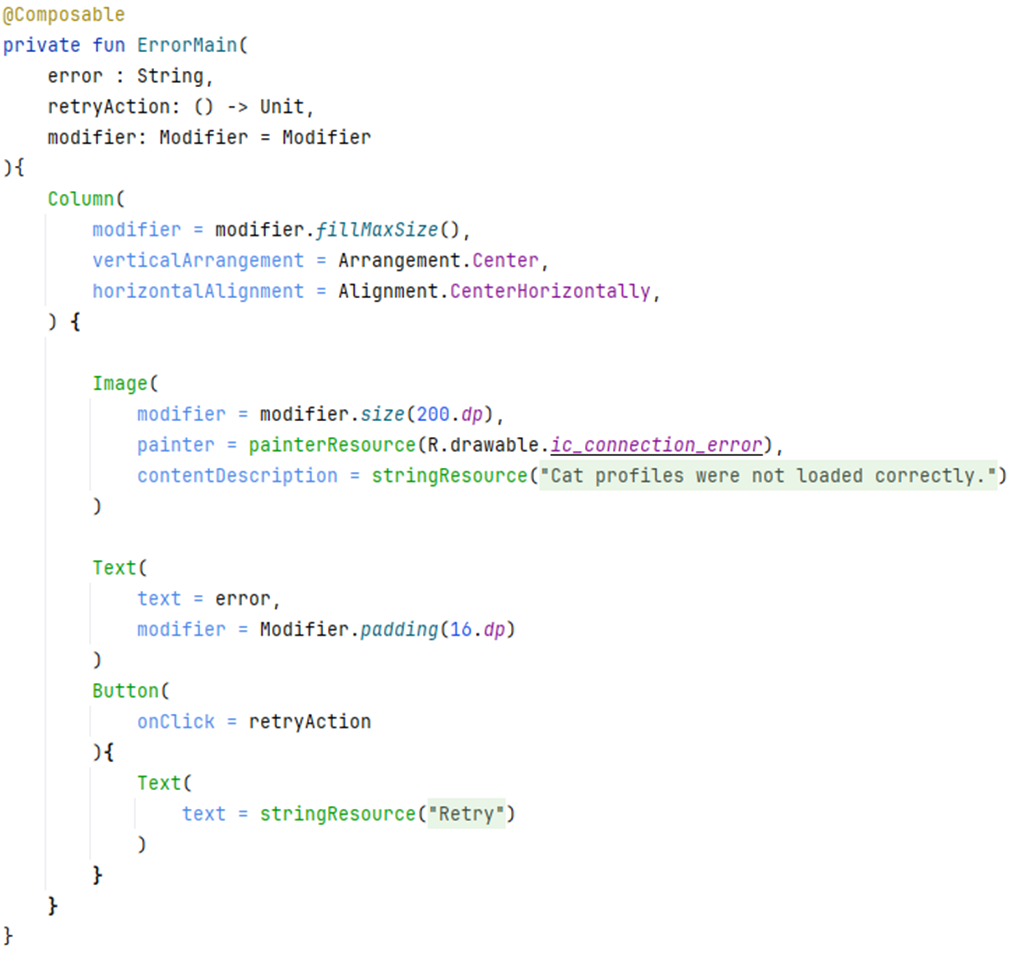
\includegraphics[scale=0.9]{MVVM_Screen}
\end{center}

\subsection{State}
State worden gebruikt om door te geven aan de UI wat te tonen. Alle nodige informatie voor de screens wordt zo gegeven.
Twee formaten worden doorheen de app gebruikt, volgens wat de context nodig heeft.
\begin{center}
    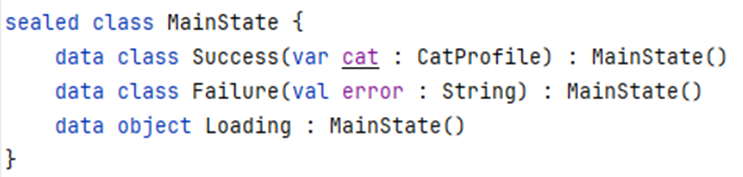
\includegraphics{MVVM_State}
\end{center}

\subsubsection{State List}
State List data classes maken gebruik van Kotlin's sterke enum types en smart casting om verschillende mogelijkheden efficiënt te behandelen, zonder extra gevallen.
Elke entry is een data class/object en heeft andere parameters. Zo weet de Screen dat een Failure entry een foutmeldingsstring bevat, terwijl een Success entry bvb. een CatProfile heeft.
De publieke constructor van de screens krijgen een state als parameter vanuit het viewmodel en lossen intern elke entry op met een aparte composable functie.

Stel er wordt externe data opgehaald door het viewmodel, en er loopt iets mis. Het viewmodel kan een Failure state inzetten met een foutmelding.
Dit belandt bij de Screen, waar een FailureScreen wordt gemaakt met de geleverde fout, die in een textvak wordt gezet.
Stel de gebruiker herlaad de pagina, maar deze keer komt de data wel correct binnen. Het viewmodel zet dan de state op Success met de State Container als parameter.
\begin{center}
    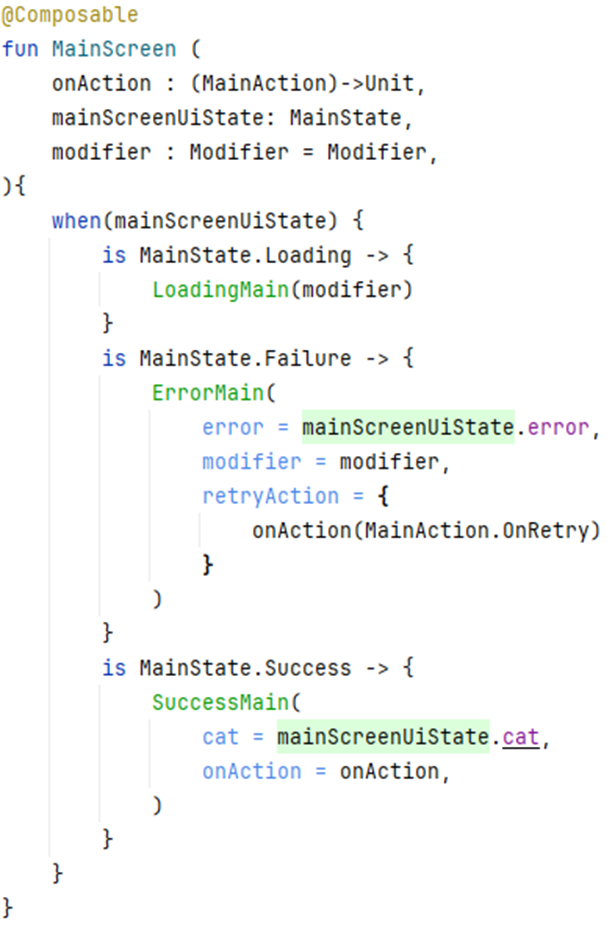
\includegraphics{MVVM_ScreenState}
\end{center}

\subsubsection{State Container}
State Containers zijn, kort door de bocht, data classes waarmee alle data voor de UI in een bundle wordt verzameld.
Zo moet er maar één parameter gegeven worden indien de UI er meerdere nodig heeft.
Dit systeem wordt niet bij elke pagina toegepast; de MainScreen heeft enkel een CatProfile nodig, verder niets.
\begin{center}
    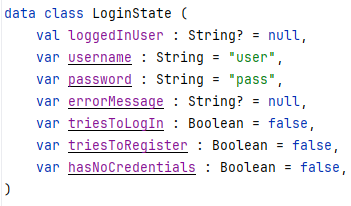
\includegraphics{MVVM_StateContainer}
\end{center}


\subsection{Action}
Terwijl State gebruikt wordt om van het viewmodel naar de UI te communiceren, Action is net het omgekeerde.
Zoals State List, Actions zijn enums (sealed classes), waardoor er makkelijk en veilig verschillende opties gemaakt kunnen worden.
Met één centrale methode in het viewmodel kunnen alle nodige acties uitgevoerd worden zonder een nieuwe parameter aan te maken voor elke interactie.
Zo wordt de code in de App file wat beperkt; het is anders makkelijk om honderden regels code te maken om alle interacties in te stellen voor elke pagina.
In het viewmodel bestaat maar één publieke methode: \textit{DoAction}, die als enige parameter een Action object van de overeenkomende type nodig heeft.
Intern worden alle scenarios behandeld en het resultaat via het de State weergegeven in de UI. 

Het beste voorbeeld hiervan is de Register pagina. Hier moet een emailadress en paswoord ingevuld worden, twee cruciale elementen van de gebruiker.
Uiteraard mag het paswoord niet te kort of simpel zijn.
Abstractie zegt dat de UI deze logika niet zelf mag uitvoeren --- wat ook erg logisch is volgens mij --- dus deze informatie moet tot het viewmodel geraken.
Aan de hand van het DoAction methode van het viewmodel, doorgegeven via de constructor van de pagina, kan OnPasswordUpdate uitgevoerd worden, met het paswoord als invoer.
Deze controleert of het voldoet en update de \textit{canSignUp} property van de State Container.

\begin{center}
    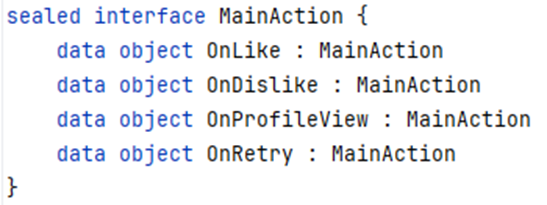
\includegraphics{MVVM_Action}
\end{center}



\section{Database}
\subsection{Optimisatie}
Data ophalen en opslaan is één van de kenmerken van hedendaagse applicaties en ligt aan de kern van een toepassing zoals deze.
Het zou een heel speciale app zijn was een netwerkverbinding niet nodig; waar zouden de katten vandaan komen?
Al gaan we er van uit dat telefoons sneller en efficiënter worden met elke nieuwe generatie, zekerheid kunnen we nooit hebben dat alle gebruikers een onbeperkte mobiele gegevens subscriptie hebben.
Er is een evenwicht te vinden tussen de hoeveelheid data die opgehaald wordt en de hoeveelheid data die lokaal verwerkt moet worden, die geregeld kan worden door meer of minder taken te geven aan de database.
Ofwel zorgt de database / server voor alle logica, filtreren en leveren van informatie, ofwel worden sommige taken aan de gebruiker overgelaten, waarbij rekenkracht voor de server bespaard wordt.
Het eerste richt zich meer op de gebruikers, door hun eventuele mobiele data subscriptie te besparen, terwijl de tweede toekomstgericht werkt;
hoe meer gebruikers, hoe meer rekenkracht de server nodig heeft, hoe sneller deze kan overlopen.


Het zou volledig mogelijk zijn om dit project op te bouwen envan uitgaand dat iedere gebruiker over onbeperkte data en de nieuwste generatie telefoon beschikt.
Dit zou mij veel moeite besparen op vlak van programmeer- en denkwerk, maar\ldots daar ben ik zelf niet tevreden mee.
Hardware stijgt razendsnel in rekenkracht en programma's kunnen groeiende hoeveelheiden resources in beslag nemen, waardoor eenvoudige taken nauwelijks merkbaar worden in de loop van de toepassing.
Verder nog, voor een toepassing met zo weinig gebruikers zullen de grootste bestanden de afbeeldingen blijven; of er twintig of hunderd gebruiker IDs opgehaald moeten worden maakt in vergelijking niks uit.
Efficiëntie-gericht programmeren geef ik voorkeur over het alternatief, maar in deze context zijn de optimisatietechnieken amper merkbaar.
De kleine stappen hiervoor bespreek ik verder wel.

\subsection{Structuur}
In dit project heb ik voor een Firebase \textit{Realtime Database} gekozen. Deze worden op een server van Google gehost en kunnen vrij grote `.json' bestanden bevatten.
Dit is de simpelste oplossing op organisatievlak, maar heeft wel een paar tekortkomingen waar rond moest dansen.
Het is een `.json' database, dus feitelijk een enkel-tekst database. Afbeeldingen kunnen niet opgeslaan worden, enkel een link er naartoe verwijzend.
Er waren een paar alternatieven die ik na onderzoek tegen was gekomen.
\begin{enumerate}
    \item Firebase heeft een subclasse, Firebase \textit{Firestore}, wat wel een relationele database is met ruimte voor afbeeldingen.
Al zou dit mijn probleem volledig oplossen, deze is niet gratis te gebruiken --- zeker door het verschil in rekenkracht met de gratis alternatief.
    \item SupaBase is een relationele database die gebruikt wordt door een paar medestudenten. Dit platform begint gratis met wat ruimte voor afbeeldingen, en wordt pas betalend eens je boven dat volume geraakt.
Al zou het een ideale oplossing zijn, ik heb die pas recent ontdekt, en Firebase was al ferm ingegroeid in de app, waardoor ik het hart niet meer had om te wissellen.
    \item Ten laatste was de optie er om zelf een simpele API te hosten met achterliggende database.
Hier zou ik volledig controle hebben over heel het infrastructuur, en zou mogelijks via een gratis URL of SSH toegang kunnen krijgen.
Het probleem hier is dat ik thuis geen extra laptop heb die permanent kan aan blijven. Dit idee ging dus volledig af te tafel.
\end{enumerate}
Één ander voordeel dat een eigen server zou brengen is dat de administratie taak volledig van de gebruiker weg kan genomen worden.
De server heeft kennis van wat elke gebruiker al heeft gezien en kan zelf profielen suggereren, \textit{wat eigenlijk één van mijn primaire doelen was}.
Dit zou op een eigen machien moeten lopen; er is geen suggestiesysteem in Subapase.
Maar ach, Firebase \textit{Realtime Database} is het geworden.

Gebruikers emails worden meestal gebruikt in het pad; deze zijn uiteraard altijd uniek en kunnen dus maar naar één gebruiker verwijzen. 
Ze worden eerst naar Base64 ge encodeert om speciale karacters te mogen gebruiken zonder conflicten met de URL.
De opslag is gesplitst in een paar regios.

\begin{enumerate}
    \item ``users'', waar de email en account-gegevens opgeslaan worden.
    Hier wordt ook informatie zoals de laatste geziene profiel bijgehouden en de profiel ID die bij het account past.
    \begin{center}
        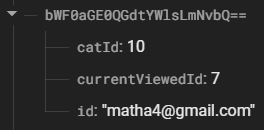
\includegraphics{DB_user}
    \end{center}

    \item ``cats'', waar de publieke informatie voor profielen te vinden is (cat id, naam, beschrijving en afbeelding link).
    Dit is wat bij elke Like / Dislike op de main pagina gezocht wordt.
    De ID's zijn bewust een integer aangezien er geen server is die zelf een profiel kan leveren; de gebruiker's apparaat moet dus zelf +1 doen om de volgende te halen.
    Dit zou niet gaan indien het ID een string is bvb.
    \begin{center}
        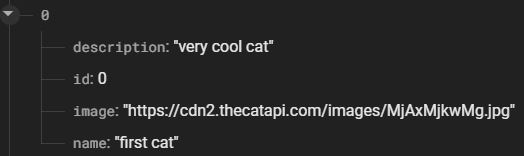
\includegraphics{DB_cat}
    \end{center}
    
    \item ``liked'', waar elk account apart onthoudt welke profielen geliked zijn en welke niet.
    Wanneer een profiel geliked wordt hun catID in de \verb|liked/user_id/l/liked_cat_id| tabel te staan.
    Disliken werkt identiek hetzelfde, alleen vervang de \verb|l| met een \verb|d|.
    \begin{center}
        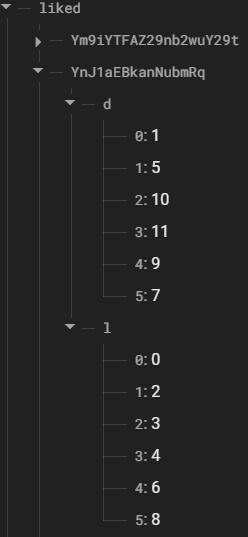
\includegraphics{DB_liked}
    \end{center}

    \item ``user\_ids'', een verbindingstabel van accounts en profielen.
    Dankzij deze voorkom ik dat de gebruiker bij het registreren \textit{alle} data van alle profielen moet ophalen.
    Hiermee kan je alle IDs krijgen, checken of je email in gebruik, checken wat de hoogste catID is en de volgende nemen.
    Zo voorkom ik dat nog de email, nog een catID twee keer gebruikt wordt.
    \begin{center}
        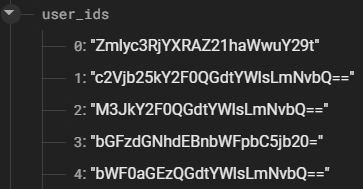
\includegraphics{DB_userids}
    \end{center}

\end{enumerate}




\section{Accounts}
De app maakt gebruik van de Android-ingebouwde Credential Manager, gemaakt en geregeld door Google.
Hiermee kan je veilig paswoorden opslaan, ophalen en verbinden aan je Google account.
Intern wordt er gebruikt gemaakt van \textit{Account Manager}, een soort viewmodel voor de Credential Manager.
Deze bevat twee publieke methodes, \verb|signIn()| en \verb|signUp()|.

In \verb|signUp()| wordt een CreateCredential methode aangeroepen die een CreatePasswordRequest bevat.
Zo komen we een nieuwe ID + Password combinatie uit en geen google account-verbinding (wat inderdaad ook kan).
Dit slaat ook de gebruiker op in de Firebase Authentication dataset, apart van de rest van alle data.
Uiteindelijk wordt nog de \verb|createUserWithEmailAndPassword()| methode aangeroepen, ingebouwd in het Firebase Authentication systeem.
\begin{center}
    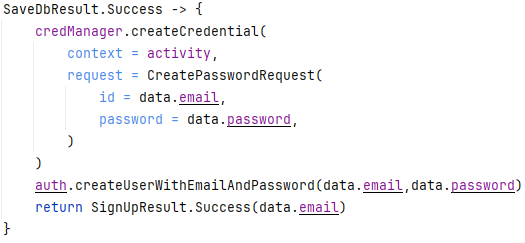
\includegraphics{ACC_Create}
\end{center}

De \verb|signIn()| functie loop best gelijk.
Hier wordt \verb|getCredential()| gebruikt in plaats van de creatie-methode, me filtering op alleen PasswordOption paswoorden.
Nogmaals, dit vermijdt dat Google-accounts opgehaald worden.

\begin{center}
    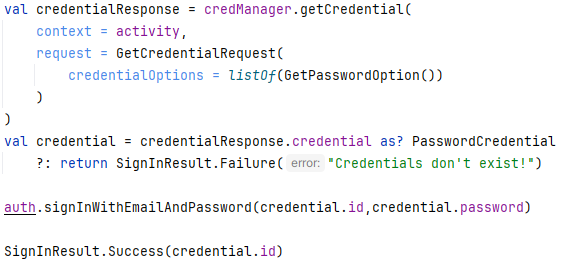
\includegraphics{ACC_Get}
\end{center}


\section{Navigatie}
De navigatiestructuur in Kotlin Jetpack Compose is niet altijd duidelijk wanneer je met de omgeving begint.
Termen zoals \textit{NavController} en \textit{NavHost} worden snel door elkaar gegooid in artikels,
iedereen heeft een andere manier van werken en zelfs Google is niet eenduidig met hoe ze het willen.
Sommige concepten blijven wel hangen, en na wat puzzlen in een ander project ben ik op deze oplossing gekomen.

Elke \textit{composable} in de Navigation Host moet een adres bevatten dat uniek hier naartoe kan lijden.
Deze adressen worden intern altijd naar een string omgevormd, maar met eenvoudige text adressen werken is niet erg praktisch.
Zie het zoals een postbode. Krijgt hij het adres, prima, maar zonder beschrijving van welke mail bij dit huis moet is hij er ook niets mee.

Daarmee komen serialiseerbare objecten/data classes van pas.
Aan de hand van de \textit{@Serializable} tag kunnen objecten serialiseerbaar worden, wat betekent dat je deze kunt omzetten (serialiseren) naar een string en vice-versa.
Een ander merkwaardige eigenschap is hoe je properties kunt aanmaken en instellen binnen een data class.
Serialiseer je er zo één, kan je data sturen doorheen de applicatie als parameters in de navigatieadressen.
\begin{center}
    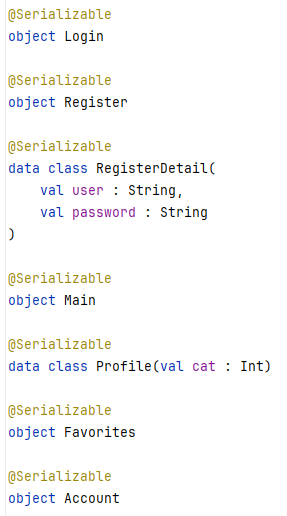
\includegraphics[scale=0.8]{NAV_Serialisable}
\end{center}

Elke van deze adressen kan je koppellen aan een \textit{composable}, om het als een effectief adress in te stellen.
Hier kan je dat object deserialiseren om de parameters uit te halen, maar uiteraard ook alle instellingen juist zetten voor de screen, zoals navigatiefuncties.
In de context van de RegisterDetails pagina dient dat om de email en passwoord ingegeven op de vorige pagina door te geven.
Deze worden uitgelezen en in de state van de nieuwe pagina onthouden.
\begin{center}
    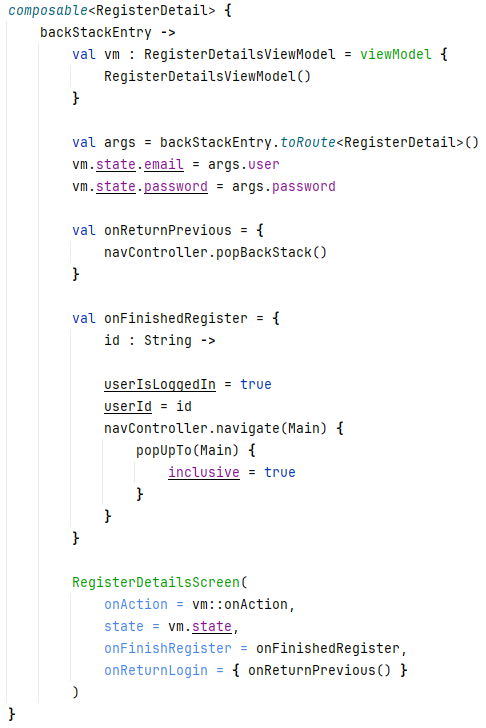
\includegraphics[scale=0.8]{NAV_Composable}
\end{center}

Verder bestaat er een \textit{Route} classe, die gebruikt wordt voor de navigatiebalk.
Hierbij moet een naam, route en icon gegeven worden.
De naam dient voor accessibility / scherm lezers in geval van mindervaliden met zichtsproblemen.
De route geeft mee naar welk adress genavigeerd moet worden, en de icon is het ikoontje dat je ziet.
\begin{center}
    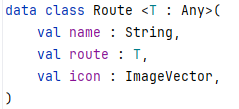
\includegraphics{NAV_Route}
\end{center}

Deze worden uiteindelijk in een lijst gezet, en mee gegeven aan de Bottom Bar.
Enkel de nodige routes komen hier te staan, uiteraard.


\chapter{Besluit}
Het maken van \textit{OnlyPaws}\texttrademark  was een leerrijkzame ervaring,
beide op vlak van programmeren als op productie-wijs redeneren.
Zelf alle kleine details uitwerken van de achterliggende code laat men appreciëren hoe veel werk er effectief zit in onze allerdaagse apps.
Al zijn de programmeertools van Google niet altijd eenduidig en helder te gebruiken, er is enorm veel moeite in gestoken om de productie van nieuwe toepassingen zo vlot mogelijk te laten lopen.

Kotlin is mijn eerste ervaring met een \textit{functional programming language}, buiten talen die er begrippen van over nemen (stel maar, Rust's Closures of C\#'s Delegates).
Ik ben niet in staat te zeggen welke stijl ik liever heb, maar ik ben wel content om de voetjes al een beetje nat te hebben gemaakt.
Één project lang diep duiken in het prullen-werk van zo een toepassing en groeiende taalomgeving is erg interessant, en kan veel bijbrengen. 

Wat ik niet opnieuw zou doen, is deze topic voor het project.
Al is ``een dating app voor katten'' wel grappig en interessant te maken, er kwam veel te veel gedoe op met afbeeldingen.
Jetpack Compose heeft hier alle nodige tools voor, maar niet altijd dicht bij de hand.
Meerdere keren moest ik een half uur terug stappen omdat ik ergens een afbeelding was vergeten een vaste grootte te zetten, of een waarde moest gokken dat er hopelijk goed zou uitzien.
Voor een eerste ervaring met de taal was het te doen, ja, maar in het vervolg zou ik zeker een project kiezen waar minder focus op afbeeldingen ligt, en voorral geen moeten opgeslaan worden.

\end{document}
